\section{Querying Interdialectal Links}

\begin{table}
{\small
\begin{tabular}{ccccc}
                & $c=1.0$   & $c\geq 0.65$  & $c \geq 0.5$  & total \\ \hline
Plautdietsch    & 834       & 1,260          & 1,416          & 3,665 \\
Plattmakers     & 1,306     & 1,676          & 1,895          & 2,433 \\
Reuter          & 1,571     & 2,107          & 2,375          & 2,835 \\
Twents          & 1,641     & 3,200          & 4,775          & 10,149\\
Westphalian     & 2,472     & 3,585          & 4,259          & 5,761 \\
\hline
\end{tabular}
} % fontsize
\caption{\emph{WöWö} links with different dictionaries, filtered by confidence scores}
\label{tab-results}
\end{table}

For evaluation, we used a single SPARQL SELECT query to retrieve all \emph{WöWö} lemma forms, their URL, (a concatenation of) their German translations, as well as aggregates (concatenations) of lemmas, confidence scores and URLs for all external dictionaries (Appendix \ref{appendix-sparql}). With this query, this information can be conveniently retrieved and exported to HTML. Both the query and its results are bundled with the release of our data and a snippet of the HTML output is shown in Fig. \ref{fig-interdialectal-links-in-html}. Note that this uses the URLs of the lexical entries (i.e., for external dictionaries, their native URL) as the basis for hyperlinks, so that all links can be interactively explored.

\begin{figure*}
    \hspace{-0.15cm}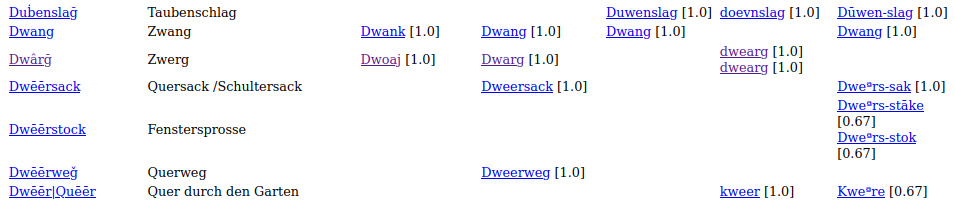
\includegraphics[width=1.025\linewidth]{img/html.png}
    \caption{Interdialectal link index, HTML export, columns from left to right: \emph{WöWö}, \emph{WöWö} translation, Plautdietsch, Plattmakers, Reuter, Twents, WWB}
    \label{fig-interdialectal-links-in-html}
\end{figure*}

On this basis, we conducted a qualitative evaluation for 50 randomly sampled links for Plattmakers and WWB (Tab. \ref{tab-eval}): 
Overall, we found the majority of links (82\% for Plattmakers, 64\% for WWB) to represent exact or approximative matches, and in line with relative proximity of Plattmakers and \emph{WöWö} varieties, with much better results for Plattmakers. One major factor for the high number of mismatches is that North Low Saxon (\emph{WöWö} and Plattmakers) normally drop unstressed Middle Low German e (apocope and syncope), whereas the Westphalian varieties (WWB and Twents) normally maintain it. 
As we cannot reliably distinguish stressed and unstressed syllables, the Westphalian (WWB and Twents) normalization allows to omit \emph{any} \word{e}, so that words like Twents \word{efn} `respectable' and \word{ven} `swampy meadow' include the same (possible) normalizations and can thus be easily confused. As we use Levenshtein distance as an additional disambiguating factor along with normalization-based confidence, dialects with apocope and syncope are likely to yield similar results, whereas the degree of variation (and the Levenshtein distance) is generally greater to dialects without apocope.

By approximative matches, we mean that either one of the words in a multi-word expression is identical, e.g., \word{Block Speck} `chunk of bacon' with Plattmakers \word{Block} `block, chunk, large piece', or that it involves a more or less transparent shift of meaning, e.g., \word{Ool} `eal' with Twents \word{Oal} (derogative nickname for persons notorious for speaking glibly), based on Twents \word{oal} `eal' (which is also linked). 
Aside from clearly incorrect links, the category of mismatches also includes homophones, e.g., WWB \word{Ō¹st} `branch' and \word{Ō²st} `east', which are historically unrelated, but formally identical (in some varieties, at least), and can thus not be disambiguated by any method of form-based matching.  We conclude that our formal linking method represents a reasonable baseline for future research to improve upon.
In particular, such improvements can be achieved if meaning relations (i.e., the glosses, definitions and translations in the respective dictionaries) are taken into account. 
For the time being, we recommend downstream applications for the cross-dialectal linking to operate with high-confidence links, only, i.e., cases in which the lack of ambiguity in the formal agreement indicates a reliable link. For the cautious user, we recommend a confidence threshold of $>0.5$, as this entails that at least one direction of the linking was formally unambiguous. 

\begin{table}
        \centering
        {\small 
        \begin{tabular}{lcc}
        & Plattmakers           & WWB \\\hline
        match                   & 0.66 (33/50) & 0.59 (29/50) \\
        approx. match     & 0.16 (8/50) & 0.06 (3/50) \\
        mismatch                & 0.18 (9/50) & 0.36 (18/50) \\
    \end{tabular}
    } % size
    \caption{Qualitative evaluation for 50 \emph{WöWö} lemmas}
    \label{tab-eval}
\end{table}

%\begin{figure}
%    \centering
%    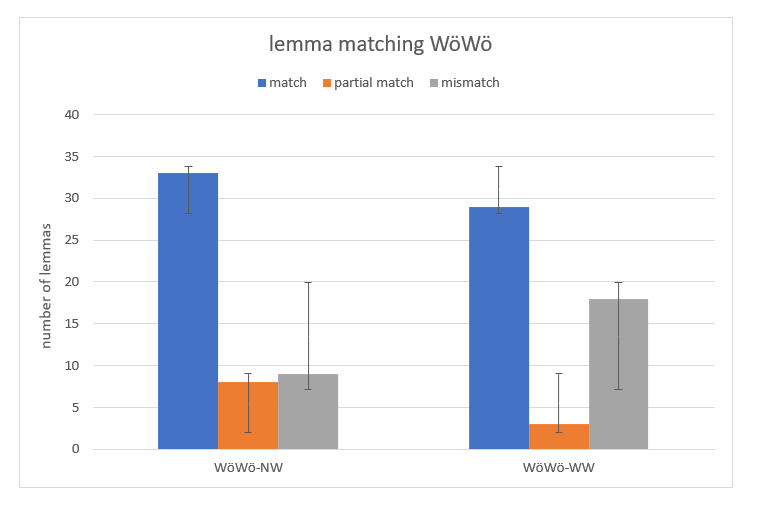
\includegraphics[width=1\linewidth]{lemma-matching-woewoe.png}
%    \caption{Qualitative evaluation over 50 \emph{WöWö} links for Plattmakers and WWB dictionaries}
%    \label{fig-eval}
%\end{figure}

The total number of links predicted for individual dictionaries is summarized in Tab. \ref{tab-results}, reporting only the most confident link for every source dictionary lemma.
In total, the linking covers 8,001 \emph{WöWö} entries, thus conforming these to be lemma forms. This number appears to be small in comparison to the 26,713 lexical entries of \emph{WöWö} in total, but to a large extent, this is due to compounds and derived forms that were included in \emph{WöWö}, but not (or, at least, not as independent lemmas) in the other dictionaries. As such, we have 41 lexical entries for \word{trecken} `to pull' and its derived forms in \emph{WöWö}, but only 18 of these have been linked. The reason is not so much that words such as \word{rantrecken} `to pull here', \word{rintrecken} `to pull inside', \word{roptrecken} `to pull up there', \word{rövertrecken} `to pull over', \word{rumtrecken} `to pull over', or \word{ruuttrecken} `to pull out' don't exist in the other varieties, but they haven't necessarily been included in the other dictionaries because their formation follows a regular and productive morphological pattern and they don't convey a semantic meaning that cannot be deduced from its parts. In fact, any locative adverb can be combined with \word{trecken} and similar verbs of motion. The same holds true for nominal compounds, which are about as productive as in High German, but are normally not included in the other dictionaries unless they have special semantics that cannot be derived from its parts.

%% mostly needed for linguists ;)
% Furthermore, the \emph{WöWö} contains a considerable number of phrasal expressions, which are not necessarily included in the other dictionaries, because these take a primary stance on documenting lexical semantics, not idiomatic expressions. The phrase \word{wat se wull, dat wull se} `what she wants, she wants' is an established idiom, but simply beyond the scope of word-centered (rather than collocation) dictionaries. Likewise, \emph{WöWö} aims to be a practical tool for the modern day, and so it includes reference translations for certain institutions which are, however, just translated word by word from their respective national language. The \word{Zentroolroot vun de Juden} `Central Council of Jews (in Germany)' mirrors German \word{Zentralrat der Juden} almost exactly, except that the German genitive has been translated as a prepositional phrase. This is necessary because the genitive case was eliminated in North Low Saxon (and other dialects with apocope), this is informative for users of the dictionary (because it gives them a reference translation), and so, this is a legit entry. However, it can also be predicted by any competent speaker from the official designation in German. It is nevertheless a legit entry to the \emph{WöWö} as a practical dictionary, because it helps its users to find appropriate expressions in cases in which there is a risk to resort to a High German loan construction (such as the genitive, in this case).

\ign{
    Beyond that, there are truly regional expressions or morphophonological processes. By comparison with its High German cognate \word{abgeordnet}, the \emph{WöWö} term \word{afornt} `delegated' can be constructed to have underlying Low German reference form like \word{*av-ordņt}. But the consonant cluster \word{ordņt} may have been a bit of a challenge to speakers, and the \emph{WöWö} entry indicates some simplification: The syllabic n has been simplified and the d has been assimilated with the r. Even though similar reduction processes exist in other dialects, as well, the specific result may be different, so that a direct 1:1 correspondence may not be found. Apocope and syncope are wide-spread phenomena in Low German, so that reduction and simplification processes are omnipresent, but with the lack of standard variety to orient towards since the demise of the Hanse, these processes produced regionally different results, and capturing them exhaustively with the FST approach pursued here would be intractable.
}